\chapter{Cadre industriel, état de l'art et données}

\chapintro
Ce chapitre situe le projet dans la maintenance industrielle, résume les méthodes de pronostic utilisées dans la littérature, puis décrit les données PRONOSTIA.

\section{Les stratégies de maintenance}

La norme NF EN 13306 \cite{nf13306} distingue trois grandes stratégies de maintenance (tableau~\ref{tab:strategies}). Notre projet relève de la maintenance \textbf{prévisionnelle} : on mesure l'état du roulement et on prévoit son évolution pour intervenir au bon moment \cite{jardine2006}.

\begin{table}[H]
\centering\small
\begin{tabularx}{\linewidth}{lYYY}
\toprule
Stratégie & Principe & Avantage & Inconvénient \\
\midrule
Corrective & on répare après la panne & rien à surveiller & arrêt imprévu, dégâts, coût élevé \\
Préventive systématique & on remplace à un âge fixé & facile à planifier & on jette des pièces encore bonnes \\
Conditionnelle et prévisionnelle & on mesure l'état et on prévoit la panne & on intervient au bon moment & capteurs, données et modèles nécessaires \\
\bottomrule
\end{tabularx}
\caption[Stratégies de maintenance (NF EN 13306)]{Les trois stratégies de maintenance (NF EN 13306).}
\label{tab:strategies}
\end{table}

\section{Cadre industriel du projet}

La norme ISO 13374 \cite{iso13374} découpe la surveillance d'une machine en six blocs de traitement. Le tableau~\ref{tab:iso} montre que notre chaîne suit ces six blocs dans l'ordre : le projet a la forme d'un vrai système industriel de surveillance, du capteur jusqu'à l'aide à la décision.

\begin{table}[H]
\centering\small
\begin{tabularx}{\linewidth}{lY}
\toprule
Bloc ISO 13374 & Dans notre projet \\
\midrule
1. Acquisition des données & 2 accéléromètres, 25,6 kHz, 0,1 s toutes les 10 s \\
2. Traitement des données & filtrage, 36 indicateurs de vibration (features) \\
3. Détection d'état & premier défaut par la règle des 3 $\sigma$ \\
4. Évaluation de la santé & indicateur de santé (HI) \\
5. Pronostic & RUL prédite par 7 méthodes, avec incertitude \\
6. Aide à la décision & quand remplacer le roulement, et combien on économise \\
\bottomrule
\end{tabularx}
\caption[Blocs de la norme ISO 13374 dans le projet]{Les six blocs de la norme ISO 13374 dans notre projet.}
\label{tab:iso}
\end{table}

\section{État de l'art}

Les méthodes de pronostic se rangent en trois familles \cite{lei2018,si2011} :
\begin{itemize}
  \item \textbf{fiabilité de la population} : une loi de durée de vie (Weibull \cite{weibull1951}) estimée sur un parc, sans capteur. Elle donne le B10 ou le MTTF, mais la même réponse pour tous les roulements ;
  \item \textbf{modèles stochastiques de dégradation} : l'indicateur de santé suit un processus aléatoire, souvent un processus de Wiener, et la RUL est le temps pour atteindre un seuil \cite{si2011,zhang2018}. Ils donnent naturellement un intervalle d'incertitude ;
  \item \textbf{modèles guidés par les données} : SVR \cite{drucker1997}, processus gaussiens \cite{rasmussen2006}, forêts aléatoires \cite{breiman2001}, puis réseaux profonds LSTM \cite{hochreiter1997} et CNN \cite{li2018cnn}, qui apprennent directement le lien entre les mesures et la RUL.
\end{itemize}
Sur PRONOSTIA, l'étude comparative récente de Dhungana et al. \cite{dhungana2025} montre que les résultats varient beaucoup d'un roulement à l'autre et que le choix de l'indicateur de santé compte autant que le modèle. Pour choisir cet indicateur, nous utilisons les critères de Coble et Hines \cite{coble2009}.

\section{Les données PRONOSTIA}

\subsection{Le banc et les conditions d'essai}
Le banc PRONOSTIA use un roulement plus vite que la normale grâce à une forte charge radiale \cite{nectoux2012}. Deux accéléromètres (horizontal et vertical) enregistrent 0,1 s de signal (2 560 points à 25,6 kHz) toutes les 10 s, et l'essai s'arrête quand la vibration dépasse 20 g. Le tableau~\ref{tab:conditions} donne les trois conditions et le découpage des roulements.

\begin{table}[H]
\centering\small
\begin{tabular}{cccll}
\toprule
Condition & Vitesse & Charge & Apprentissage (complets) & Test (arrêtés avant la fin) \\
\midrule
1 & 1 800 tr/min & 4 000 N & Bearing1\_1, Bearing1\_2 & Bearing1\_3 à Bearing1\_7 \\
2 & 1 650 tr/min & 4 200 N & Bearing2\_1, Bearing2\_2 & Bearing2\_3 à Bearing2\_7 \\
3 & 1 500 tr/min & 5 000 N & Bearing3\_1, Bearing3\_2 & Bearing3\_3 \\
\bottomrule
\end{tabular}
\caption[Conditions opératoires et découpage des roulements]{Conditions opératoires et découpage des 17 roulements.}
\label{tab:conditions}
\end{table}

\subsection{Différents types d'essais}
En fiabilité, on ne traite pas de la même façon un essai qui va jusqu'à la panne et un essai arrêté avant (tableau~\ref{tab:essais}). Les 11 roulements de test sont des \textbf{données censurées à droite} : on sait seulement qu'ils fonctionnaient encore à l'instant de troncature du challenge. L'estimateur de Kaplan-Meier \cite{kaplan1958} et le maximum de vraisemblance savent utiliser cette information.

\begin{table}[H]
\centering\small
\begin{tabularx}{\linewidth}{lYY}
\toprule
Type d'essai & Définition & Dans nos données \\
\midrule
Essai complet & on attend la panne & les 6 roulements d'apprentissage \\
Essai censuré à droite & on arrête à une date fixée à l'avance, avant la panne & les 11 roulements de test, arrêtés à la troncature \\
Essai accéléré & on use plus vite avec une charge forte & tout le banc (4 000 à 5 000 N) \\
\bottomrule
\end{tabularx}
\caption[Types d'essais présents dans les données]{Les types d'essais présents dans les données.}
\label{tab:essais}
\end{table}

\subsection{Contrôle qualité}
Aucun fichier n'est incomplet et aucune valeur ne manque. Bearing1\_1 contient 3 horodatages incohérents : le temps est reconstruit à partir du numéro du fichier (10 s par fichier). Pour Bearing1\_4, la RUL officielle (339 s) ne correspond pas au nombre de fichiers (2 890 s) : c'est une erreur connue du jeu de données, et nous gardons la valeur officielle pour le score du challenge. La figure~\ref{fig:durees} montre la grande dispersion des durées de vie : de 38 à 467 min, même sous une même condition.

\begin{figure}[H]
\centering
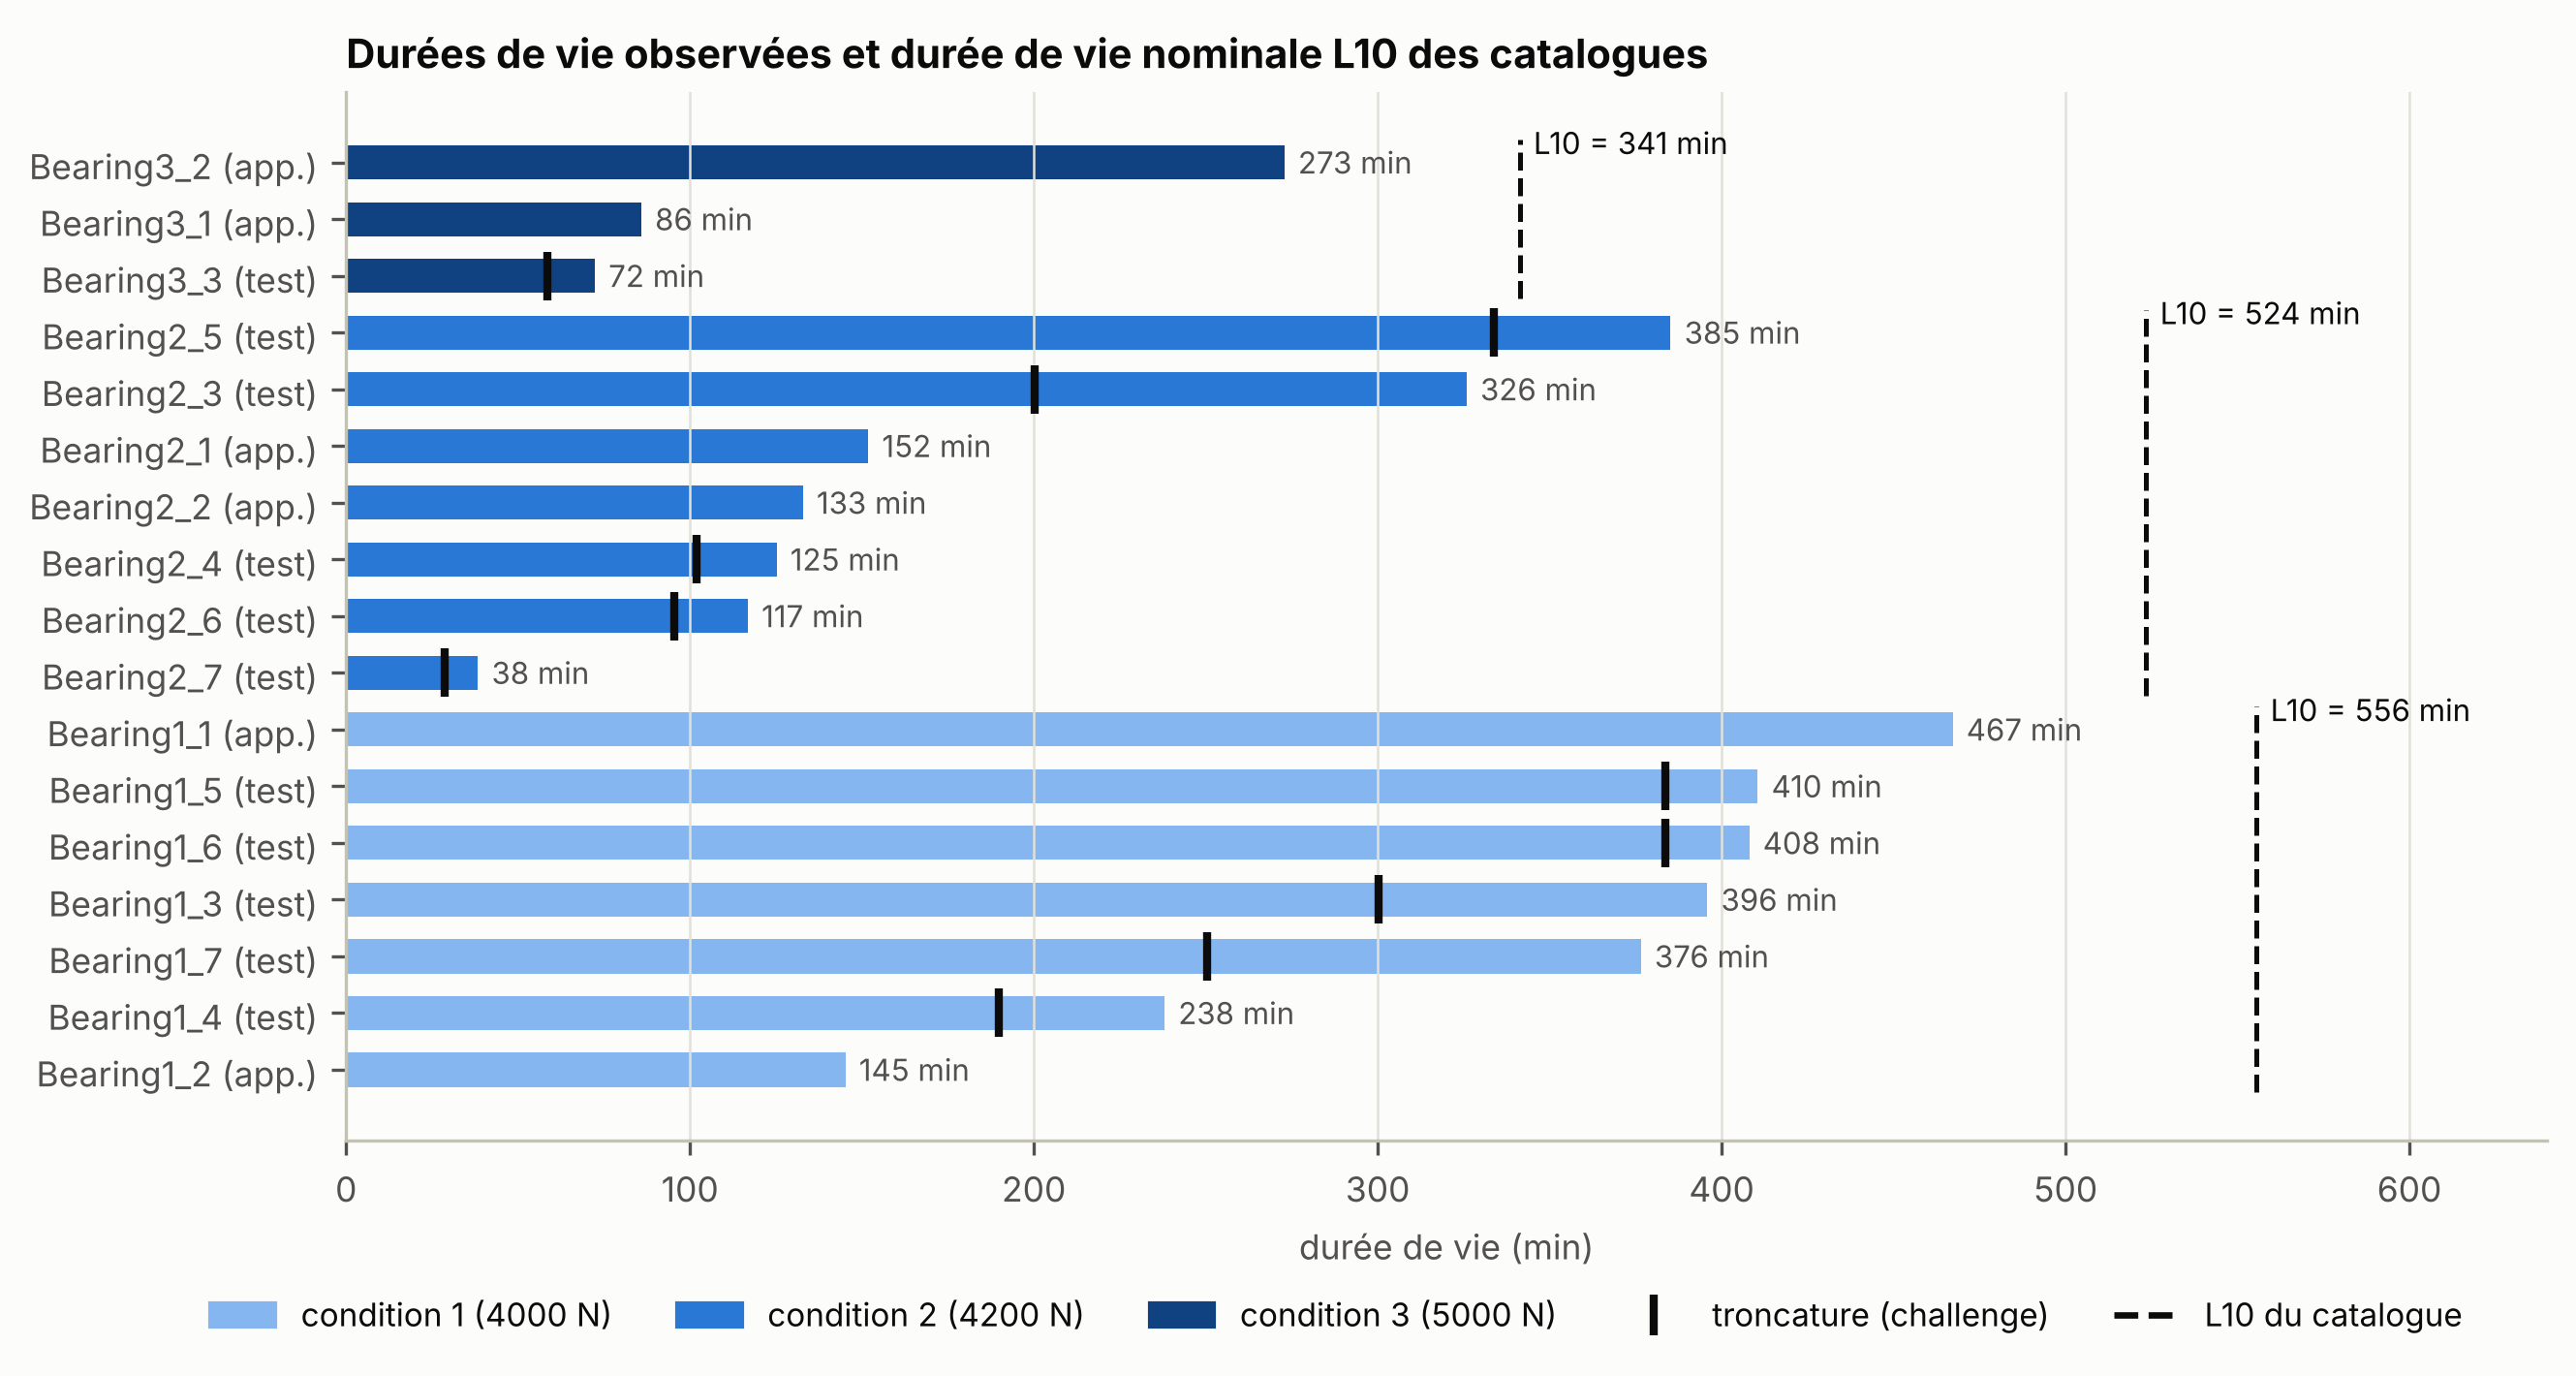
\includegraphics[width=0.8\linewidth]{figures/fig03_durees_de_vie.png}
\caption[Durées de vie des 17 roulements]{Durées de vie des 17 roulements, instants de troncature du challenge et durée L10 des catalogues.}
\label{fig:durees}
\end{figure}

\chapconclusion
Le projet suit la chaîne industrielle de la norme ISO 13374 et s'appuie sur les trois familles de méthodes de la littérature. Les données sont réelles, peu nombreuses (17 roulements) et très dispersées : il faudra être prudent dans les conclusions.
